\documentclass[xetex,mathserif,serif]{beamer}
\usepackage{polyglossia}
\setdefaultlanguage[babelshorthands=true]{russian}
\usepackage{minted}
\usepackage{tabu}
\usepackage[11pt]{moresize}

\usepackage{textpos}
\setlength{\TPHorizModule}{1cm}
\setlength{\TPVertModule}{1cm}

\useoutertheme{infolines}

\usepackage{fontspec}
\setmainfont{FreeSans}
\newfontfamily{\russianfonttt}{FreeSans}

\tabulinesep=0.7mm

\newcommand{\attribution}[1] {
    \begin{flushright}\begin{scriptsize}\textcolor{gray}{\textcopyright\; #1}\end{scriptsize}\end{flushright}
}

\title{Лекция 14: Проектирование распределённых приложений}
\subtitle{Часть вторая: стратегические вопросы}
\author[Юрий Литвинов]{Юрий Литвинов\\\small{\textcolor{gray}{y.litvinov@spbu.ru}}}

\date{14.12.2021}

\begin{document}

    \frame{\titlepage}

    \section{REST}

    \begin{frame}
        \frametitle{Representational State Transfer (REST)}
        \begin{itemize}
            \item Модель клиент-сервер
            \item Отсутствие состояния
            \item Кэширование
            \item Единообразие интерфейса
            \item Как правило, очень простые запросы
        \end{itemize}
    \end{frame}

    \begin{frame}
        \frametitle{Интерфейс сервиса}
        \begin{itemize}
            \item Коллекции
            \begin{itemize}
                \item \url{http://api.example.com/resources/}
            \end{itemize}
            \item Элементы
            \begin{itemize}
                \item \url{http://api.example.com/resources/item/17}
            \end{itemize}
            \item HTTP-методы
            \begin{itemize}
                \item GET
                \item PUT
                \item POST
                \item DELETE
            \end{itemize}
            \item Передача параметров прямо в URL
            \begin{itemize}
                \item \url{http://api.example.com/resources?user=me&access_token=ASFQF}
            \end{itemize}
        \end{itemize}
    \end{frame}

    \begin{frame}
        \frametitle{Пример, Google Drive REST API}
        \begin{itemize}
            \item GET https://www.googleapis.com/drive/v2/files --- список всех файлов
            \item GET https://www.googleapis.com/drive/v2/files/fileId --- метаданные файла по его Id
            \item POST https://www.googleapis.com/upload/drive/v2/files — загрузить новый файл
            \item PUT https://www.googleapis.com/upload/drive/v2/files/fileId --- обновить файл
            \item DELETE https://www.googleapis.com/drive/v2/files/fileId --- удалить файл
        \end{itemize}
    \end{frame}

    \section{Микросервисы}

    \begin{frame}
        \frametitle{Микросервисы}
        \begin{itemize}
            \item Набор небольших сервисов
            \begin{itemize}
                \item Разные языки и технологии
            \end{itemize}
            \item Каждый в собственном процессе
            \begin{itemize}
                \item Независимое развёртывание
                \item Децентрализованное управление
            \end{itemize}
            \item Легковесные коммуникации
        \end{itemize}
    \end{frame}

    \begin{frame}
        \frametitle{Монолитные приложения}
        \begin{itemize}
            \item Единый процесс разработки и стек технологий
            \item Существенно меньше затрат на передачу данных между компонентами
            \item Существенно проще развёртывание
            \item Невозможно масштабирование по частям
        \end{itemize}
    \end{frame}

    \begin{frame}
        \frametitle{Разбиение на сервисы}
        \begin{center}
            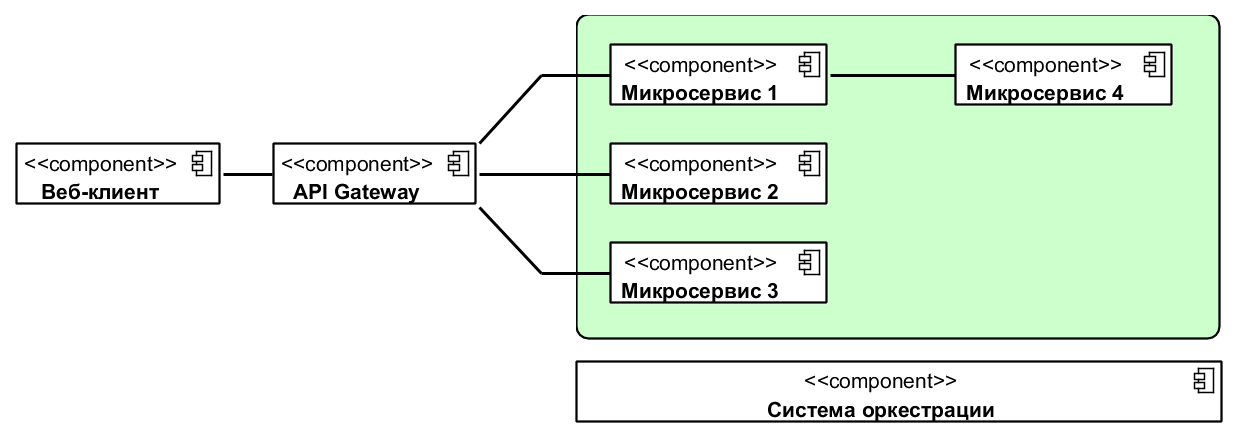
\includegraphics[width=\textwidth]{microservices.png}
        \end{center}
    \end{frame}

    \begin{frame}
        \frametitle{Основные особенности}
        \begin{itemize}
            \item Микросервисы и SOA
            \item Smart endpoints and dumb pipes
            \item Проектирование под отказ
            \item Асинхронные вызовы
            \item Децентрализованное управление данными
            \item Автоматизация инфраструктуры
            \item Эволюционный дизайн
        \end{itemize}
    \end{frame}

    \begin{frame}
        \frametitle{Основные проблемы}
        \begin{itemize}
            \item Сложности выделения границ сервисов
            \item Перенос логики на связи между сервисами
            \begin{itemize}
                \item Большой обмен данными
                \item Нетривиальные зависимости
            \end{itemize}
            \item Нетривиальная инфраструктура
            \item Нетривиальная переиспользуемость кода
        \end{itemize}
    \end{frame}

    \section{Peer-to-peer}

    \begin{frame}
        \frametitle{Архитектура Peer-to-Peer}
        \begin{itemize}
            \item Децентрализованный и самоорганизующийся сервис
            \item Динамическая балансировка нагрузки
            \begin{itemize}
                \item Вычислительные ресурсы
                \item Хранилища данных
            \end{itemize}
            \item Динамическое изменение состава участников
        \end{itemize}
    \end{frame}

    \begin{frame}
        \frametitle{Skype: Overlayed P2P}
        \begin{center}
            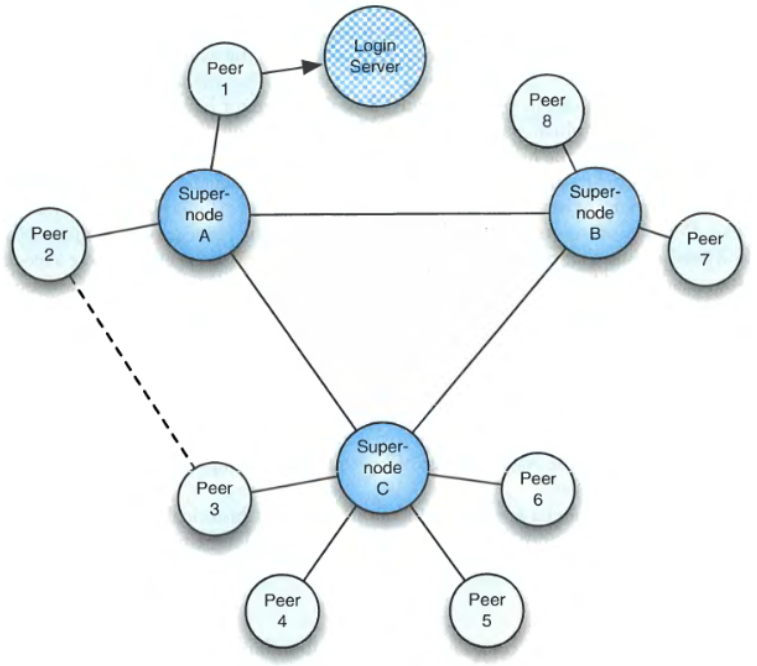
\includegraphics[width=0.6\textwidth]{skype.png}
        \end{center}
    \end{frame}

    \begin{frame}
        \frametitle{BitTorrent : Resource Trading P2P}
        \begin{itemize}
            \item Обмен сегментами
            \item Поиск не входит в протокол
            \item Трекеры
            \item Метаданные
            \item Управление приоритетами
            \item Бестрекерная реализация
        \end{itemize}
    \end{frame}

    \section{Docker}

    \begin{frame}
        \frametitle{Docker}
        \begin{itemize}
            \item Средство для ``упаковки'' приложений в изолированные контейнеры
            \item Что-то вроде легковесной виртуальной машины
            \item \item Широкий инструментарий: DSL для описания образов, публичный репозиторий, поддержка оркестраторами
        \end{itemize}
        \begin{center}
            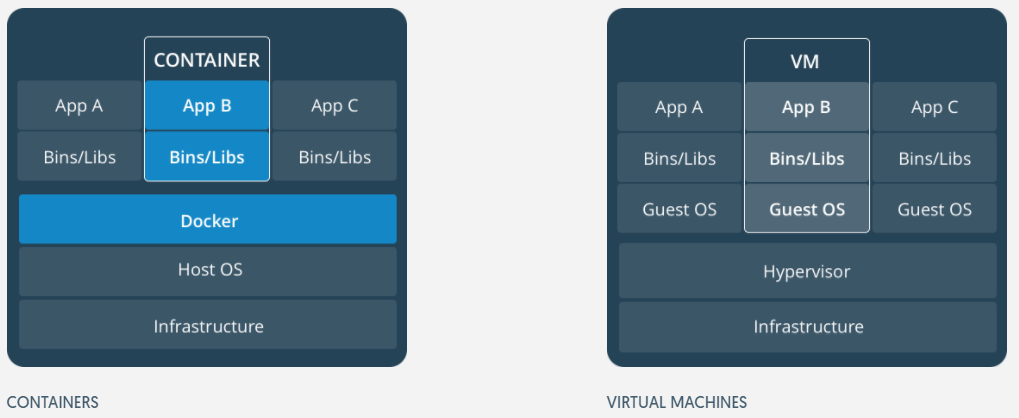
\includegraphics[width=0.7\textwidth]{docker.png}
            \attribution{\url{https://www.docker.com}}
        \end{center}
    \end{frame}

    \begin{frame}
        \frametitle{Docker Image}
        \begin{columns}
            \begin{column}{0.6\textwidth}
                \begin{itemize}
                    \item Окружение и приложение
                    \item Состоит из слоёв
                    \begin{itemize}
                        \item Все слои read-only
                        \item Образы делят слои между собой как процессы делят динамические библиотеки
                    \end{itemize}
                    \item На основе одного образа можно создать другой
                \end{itemize}
            \end{column}
            \begin{column}{0.4\textwidth}
                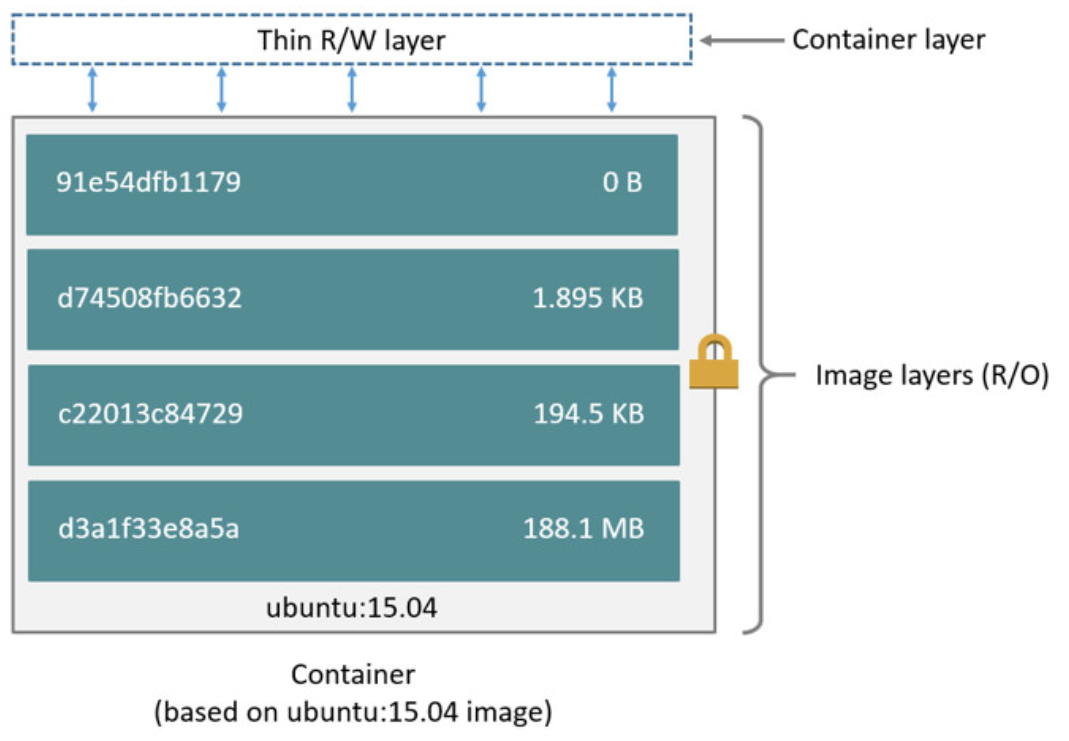
\includegraphics[width=0.9\textwidth]{dockerLayers.png}
            \end{column}
        \end{columns}
    \end{frame}

    \begin{frame}
        \frametitle{Docker Container}
        \begin{columns}
            \begin{column}{0.5\textwidth}
                \begin{itemize}
                    \item Образ с дополнительным write слоем
                    \item Содержит один запущенный процесс
                    \item Может быть сохранен как новый образ
                \end{itemize}
            \end{column}
            \begin{column}{0.5\textwidth}
                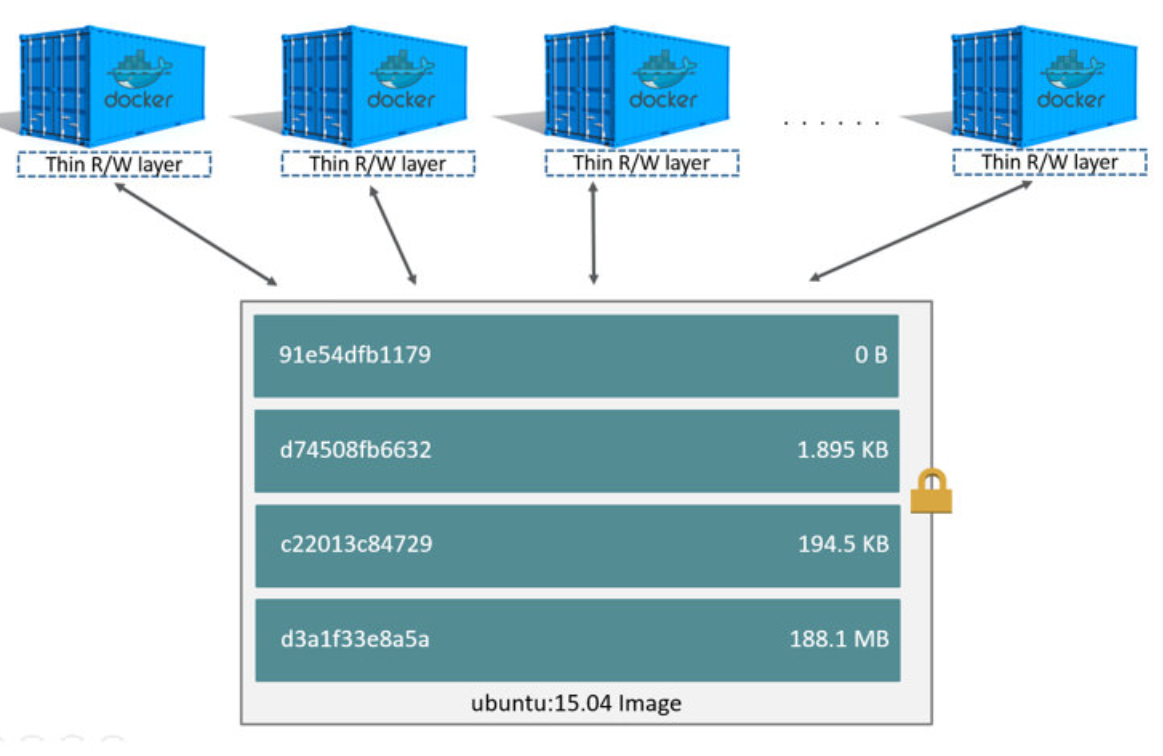
\includegraphics[width=0.9\textwidth]{dockerContainer.png}
            \end{column}
        \end{columns}
    \end{frame}

    \begin{frame}
        \frametitle{DockerHub}
        \begin{columns}
            \begin{column}{0.5\textwidth}
                \begin{itemize}
                    \item Внешний репозиторий образов
                    \begin{itemize}
                        \item Официальные образы
                        \item Пользовательские образы
                        \item Приватные репозитории
                    \end{itemize}
                    \item Простой CI/CD
                    \item Высокая доступность
                \end{itemize}
            \end{column}
            \begin{column}{0.5\textwidth}
                
\includegraphics[width=0.9\textwidth]{dockerHub.png}
            \end{column}
        \end{columns}
    \end{frame}

    \begin{frame}
        \frametitle{Базовые команды}
        \begin{itemize}
            \item docker run --- запускает контейнер (при необходимости делает pull)
            \begin{itemize}
                \item -d --- запустить в фоновом режиме
                \item -p host\_port:container\_port --- прокинуть порт из контейнера на хост
                \item -i -t --- запустить в интерактивном режиме
                \item Пример: \mintinline{text}|docker run -it ubuntu /bin/bash|
            \end{itemize}
            \item docker ps --- показывает запущенные контейнеры
            \begin{itemize}
                \item Пример: \mintinline{text}|docker run -d nginx; docker ps|
            \end{itemize}
            \item docker stop --- останавливает контейнер (шлёт SIGTERM, затем SIGKILL)
            \item docker exec --- запускает дополнительный процесс в контейнере
        \end{itemize}
    \end{frame}

    \begin{frame}[fragile]
        \frametitle{Dockerfile}
        \begin{scriptsize}
            \begin{minted}{sh}
# Use an official Python runtime as a parent image
FROM python:2.7-slim

# Set the working directory to /app
WORKDIR /app

# Copy the current directory contents into the container at /app
ADD . /app

# Install any needed packages specified in requirements.txt
RUN pip install --trusted-host pypi.python.org -r requirements.txt

# Make port 80 available to the world outside this container
EXPOSE 80

# Define environment variable
ENV NAME World

# Run app.py when the container launches
CMD ["python", "app.py"]
            \end{minted}
        \end{scriptsize}
    \end{frame}

    \begin{frame}[fragile]
        \frametitle{Балансировка нагрузки}
        \framesubtitle{docker-compose.yml}
        \begin{scriptsize}
            \begin{minted}{yaml}
version: "3"
services:
    web:
        # replace username/repo:tag with your name and image details
        image: username/repo:tag
        deploy:
            replicas: 5
            resources:
                limits:
                    cpus: "0.1"
                    memory: 50M
            restart_policy:
                condition: on-failure
        ports:
            - "80:80"
        networks:
            - webnet
networks:
    webnet:
            \end{minted}
        \end{scriptsize}
    \end{frame}

    \begin{frame}
        \frametitle{Swarm-ы}
        \begin{itemize}
            \item Машина, на которой запускается контейнер, становится главной
            \item Другие машины могут присоединяться к swarm-у и получать копию контейнера
            \item Docker балансирует нагрузку по машинам
        \end{itemize}
        \begin{center}
            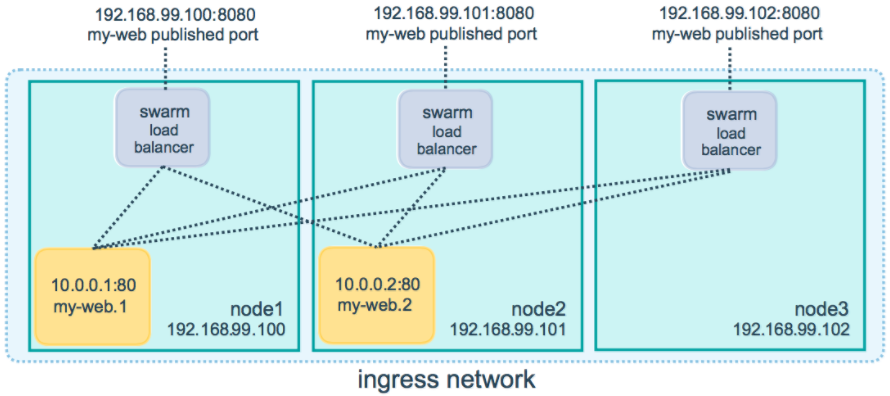
\includegraphics[width=0.7\textwidth]{swarmLoadBalancing.png}
            \attribution{\url{https://www.docker.com}}
        \end{center}
    \end{frame}

    \section{Kubernetes}

\end{document}
